\documentclass[11pt]{article}
\usepackage{acl2016}
\usepackage{amsmath}
\usepackage{times}
\usepackage{latexsym}
\usepackage{color}
\usepackage{booktabs}
\usepackage{subfig}
\usepackage{tikz}
\usetikzlibrary{bayesnet}

\newcommand{\secref}[1]{Section~\ref{sec:#1}}
\newcommand{\figref}[1]{Figure~\ref{fig:#1}}
\newcommand{\algref}[1]{Algorithm~\ref{alg:#1}}
\newcommand{\tabref}[1]{Table~\ref{tab:#1}}
\newcommand{\mattnote}[1]{\textcolor{red}{NOTE: #1}}
\newcommand{\blank}{\underline{\hspace{.5cm}}}
\newcommand{\lexicalpredicate}[1]{\ensuremath{\textit{#1}}}
\newcommand{\formalpredicate}[1]{\ensuremath{\textsc{#1}}}
\newcommand{\entity}[1]{\ensuremath{\textsc{#1}}}

\newcommand{\true}[0]{\formalpredicate{true}}
\newcommand{\false}[0]{\formalpredicate{false}}

%\aclfinalcopy % Uncomment this line for the final submission
%\def\aclpaperid{***} %  Enter the acl Paper ID here

\title{Combining Formal and Distributional Models of Predicate Semantics}

\author{}%Matt Gardner and Jayant Krishnamurthy\\
%Allen Institute for Artificial Intelligence\\
%Seattle, Washington, USA\\
%{\tt \{mattg,jayantk\}@allenai.org}}

\date{}

\begin{document}

\maketitle

\begin{abstract}

  We consider the problem of learning models of predicate (category and
  relation) semantics using both distributional information and structured
  information contained in a formal knowledge base.  Most previous approaches
  to modeling predicate semantics have either been purely distributional (such
  as word2vec and knowledge base embedding methods) or purely formal (such as
  most semantic parsers).  Distributional approaches have very broad coverage,
  but lack the compositional, logical semantics used by semantic parsers, and
  it has so far been difficult to combine the benefits of both of these
  techniques.

  In this paper, we present a method that incorporates logical statements
  derived from a knowledge base into distributional models of categories and
  relations.  Instead of mapping a phrase to a single logical statement, as
  done by semantic parsers, our method uses logical statements as features
  added to distributional models of words, allowing the model to learn that
  Freebase entities that are "honchos" are people, not buildings, and that they
  are frequently CEOs or film producers.  We use these models in an
  open-vocabulary semantic parsing task, showing a 62\% relative improvement in
  mean average precision over a distributional-only model.

\end{abstract}

\section{Introduction}

How should a computer program represent the meaning of a word or a
phrase? Recent work has suggested two vastly different
approaches---distributional vector space models and semantic
parsing---each with its own advantages and disadvantages. On one hand,
distributional models produce a vector representation of the meaning
of each word from a large unlabeled text corpus. These models have
broad coverage but a shallow semantics centered around word
similarity. On the other hand, semantic parsing translates natural
language into logical queries against a formal knowledge base, such as
Freebase. This approach produces a rich compositional semantics and
furthermore can leverage structured information from the knowledge
base, e.g., to answer natural language questions. However, semantic
parsers have limited coverage as they can only represent the meanings
of words that can be mapped to knowledge base predicates. A critical
question is \emph{how do we obtain the benefits of both approaches?}

\begin{figure*}[ht]
  \small
  \begin{minipage}{0.28\linewidth}
    \textbf{Input Text}\\Italian architect \blank{}
  \end{minipage}
%
  ~~ $\rightarrow$ ~~~~~~
%
  \begin{minipage}{0.7\linewidth}
    \textbf{Logical Form}\\
    $\lexicalpredicate{architect}(x)~\land~\lexicalpredicate{architect\_N/N}(\entity{Italy}, x)$
  \end{minipage}

  \vspace{.2in}
  \begin{minipage}{0.5\linewidth}
    \textbf{Category models}\\
    \begin{tabular}{@{}lll}
      \lexicalpredicate{architect}: & $\theta$: &[.2, -.6, \ldots] \\
      & $\omega$: & \textsc{type:architect} $\rightarrow$ .52 \\
      &           & \textsc{type:designer} $\rightarrow$ .32 \\
      &           & \textsc{nationality:Italy} $\rightarrow$ .20 \\
      &           & $\cdots$
    \end{tabular}
  \end{minipage}
  \begin{minipage}{0.5\linewidth}
    \textbf{Relation models}\\
    \begin{tabular}{@{}lll}
      \lexicalpredicate{architect\_N/N}: & $\theta$: &[-.9, .1, \ldots] \\
      & $\omega$: & \textsc{/person/nationality\textsuperscript{-1}} $\rightarrow$ .29 \\
      &           & \textsc{/structure/architect} $\rightarrow$ .11 \\
      &           & \textsc{/person/ethnicity\textsuperscript{-1}} $\rightarrow$ .05 \\
      &           & $\cdots$
    \end{tabular}
  \end{minipage}

  \begin{minipage}{0.5\linewidth}
    \textbf{Entity models}\\
    \begin{tabular}{@{}lll}
      \entity{Palladio}: & $\phi$: &[.15, -.8, \ldots] \\
      & $\psi$: & \textsc{type:architect} $\rightarrow$ 1 \\
      &           & \textsc{nationality:Italy} $\rightarrow$ 1 \\
      &           & $\cdots$ \\
      \entity{Obama}: & $\phi$: &[.85, .1, \ldots] \\
      & $\psi$: & \textsc{type:politician} $\rightarrow$ 1 \\
      &           & \textsc{nationality:Italy} $\rightarrow$ 0 \\
      &           & $\cdots$
    \end{tabular}
  \end{minipage}
  \begin{minipage}{0.5\linewidth}
    \textbf{Entity pair models}\\
    \begin{tabular}{@{}lll}
      \entity{(Italy, Palladio)}: & $\phi$: &[-.8, .2, \ldots] \\
      & $\omega$: & \textsc{/person/nationality\textsuperscript{-1}} $\rightarrow$ 1 \\
      &           & \textsc{/structure/architect} $\rightarrow$ 0 \\
      &           & $\cdots$ \\
      \entity{(Italy, Obama)}: & $\phi$: &[-.2, -.2, \ldots] \\
      & $\omega$: & \textsc{/person/nationality\textsuperscript{-1}} $\rightarrow$ 0 \\
      &           & \textsc{/structure/architect} $\rightarrow$ 0 \\
      &           & $\cdots$
    \end{tabular}
  \end{minipage}

  \begin{minipage}{0.5\linewidth}
    \textbf{Output}\\
    \begin{tabular}{@{}ll}
      $\mathrm{prob}(\entity{Palladio})$: & 0.79 \\
      $\mathrm{prob}(\entity{Obama})$: & 0.01 \\
      $\cdots$ \\
    \end{tabular}
  \end{minipage}

  \vspace{-.1in}
  \caption{Overview of the components of our model.  Given an input
  text, we use a CCG parser and an entity linker to produce a logical
  form that is a conjunction of predicates involving the entities in
  the text.  For each predicate (both categories and relations), we
  learn a distributional vector $\theta$, as well as weights $\omega$
  associated with formal features from Freebase (which are shortened
  to fit in the figure).  For each entity and entity pair, we also
  learn a distributional vector $\phi$, and we extract a feature
  vector $\psi$ from Freebase.  These models are combined to assign a
  probability to candidate entities, assigning a high probability to
  \entity{Andrea Palladio} and a low probability to \entity{Barack
  Obama}.}
  \label{fig:overview}
  \vspace{-.1in}
\end{figure*}

Krishnamurthy and
Mitchell~\shortcite{krishnamurthy-2015-semparse-open-vocabulary}
provide a partial answer to this question with their open-vocabulary
semantic parser. This system answers compositional, fill-in-the-blank
natural language queries against Freebase, such as ``Hollywood honcho
\blank{},'' using \emph{distributional} models of predicate
semantics. The method semantically parses text to a surface logical
form containing predicates derived from the text itself, such as
$\lambda x.\lexicalpredicate{honcho}(x) \land
\lexicalpredicate{honcho\_N/N}(\entity{Hollywood}, x)$, then learns the
denotations of these predicates using distributional information from
a large, entity-linked corpus. This method combines the broad coverage
of distributional approaches with the compositionality of semantic
parsing; however, it does not use structured information from Freebase
to assist with its predictions.

In this work, we introduce new models of predicate semantics that
leverage both structured information from Freebase and distributional
information. Our key observation is that, while there is no Freebase
predicate that corresponds exactly to the meaning of ``honcho,''
Freebase \emph{does} contain predicates that \emph{partially}
represent its meaning. For example, an entity that can be called
``honcho'' is likely to have type \formalpredicate{person}. We therefore
incorporate \emph{features} based on Freebase paths into the predicate
models of K\&M and learn per-predicate weights for these features
using distributional information (\figref{overview}). This approach
effectively learns the meaning of a word as a distributional vector
plus a \emph{weighted combination of Freebase queries}, a considerably
more expressive representation than either existing semantic parsers
or K\&M.

We demonstrate our approach on the task of answering fill-in-the-blank
natural language queries, finding that our approach provides a 62\%
relative improvement in mean average precision over K\&M. (TODO: other
empirical findings? It would be nice to talk about what features get
learned for what words, etc.)

\section{Background}
\label{sec:background}

In this work, we make heavy use of the open-vocabulary semantic parser
of Krishnamurthy and
Mitchell~\shortcite{krishnamurthy-2015-semparse-open-vocabulary}, as
well as features derived from a knowledge base using a technique
called subgraph feature extraction~\cite[SFE]{gardner-2015-sfe}.
Accordingly, in this section we briefly describe both of these
techniques.

\subsection{Open-vocabulary semantic parsing}
\label{sec:jayant-semparse}

Krishnamurthy and
Mitchell~\shortcite{krishnamurthy-2015-semparse-open-vocabulary}
introduced a technique for learning semantic parsers with open
predicate vocabularies (hereafter referred to as K\&M). Instead of
mapping text directly to Freebase queries, this method parses text to
a surface logical form whose predicates are derived directly from the
words in the text. Next, a distribution over denotations for each
predicate is learned using a matrix factorization approach similar to
that of Riedel et
al.~\shortcite{riedel-2013-mf-universal-schema}. This distribution is
concisely represented using a probabilistic database, which also
enables efficient probabilistic execution of logical form queries.

The truth probability of a predicate instance such as
\lexicalpredicate{architect}(\entity{AndreaPalladio}) is learned using
probabilistic matrix factorization. This factorization has two sets of
parameters: each category or relation has a learned $k$-dimensional
embedding $\theta$, and each entity or entity pair has a learned
embedding $\phi$. The probability assigned to a category instance
$c(e)$ or relation instance $r(e_1, e_2)$ is given by:

\begin{align*}
  P(c(e)) &= \sigma ( \theta_c^T \phi_e ) \\
  P(r(e_1, e_2)) &= \sigma ( \theta_r^T \phi_{(e_1, e_2)} )
\end{align*}

The probability of a predicate instance is the (sigmoided) inner
product of the corresponding predicate and entity embeddings. Thus,
predicates with nearby embeddings will have similar distributions over
the entities in their denotation. The parameters $\theta$ and $\phi$
are learned using a query ranking objective that optimizes them to
rank entities observed in the denotation of a logical form above
unobserved entities. Note that this approach is similar to modern
techniques for constructing word embeddings in that it factors a
cooccurrence matrix between predicates and
entities~\cite{levy-2014-w2v-as-mf}. Given the trained predicate and
entity parameters, the system is capable of efficiently computing the
marginal probability that an entity is an element of a logical form's
denotation using approximate inference algorithms for probabilistic
databases.

This paper extends K\&M by modifying the models of predicate semantics
as described in \secref{method}. K\&M introduced several variations of
their parser; in this work, we use their query ranking objective, as
it had the best performance, and we compare against the model they
called ``Factorization,'' without ensembling it with a corpus lookup
baseline.

\subsection{Subgraph feature extraction}

\begin{figure}
  {\center
  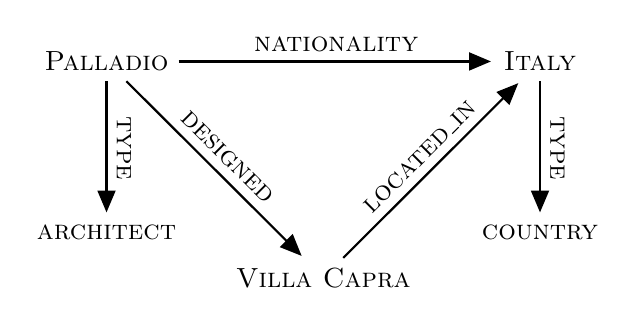
\begin{tikzpicture}[
    ->,
    shorten >=1pt,
    auto,
    node distance=3cm,
    thick,
    main node/.style={draw=none,fill=none}
    ]

    \node[main node] (1) {\entity{Palladio}};
    \node[main node] (2) [right=4cm of 1] {\entity{Italy}};
    \node[main node] (3) [below=1.7cm of 1] {\entity{architect}};
    \node[main node] (4) [below=1.7cm of 2] {\entity{country}};
    \node[main node] (5) [below right=.1cm and .5cm of 3] {\entity{Villa Capra}};

    \path[]
      (1) edge node [sloped, anchor=center, above] {\formalpredicate{nationality}} (2)
      (1) edge node [sloped, anchor=center, above] {\formalpredicate{type}} (3)
      (1) edge node [sloped, anchor=center, above] {\formalpredicate{designed}} (5)
      (2) edge node [sloped, anchor=center, above] {\formalpredicate{type}} (4)
      (5) edge node [sloped, anchor=center, above] {\formalpredicate{located\_in}} (2);
  \end{tikzpicture}
  }
  \textbf{Features between \entity{Palladio} and \entity{Italy}}:\\
  \textless\formalpredicate{nationality}\textgreater\\
  \textless\formalpredicate{designed}, \formalpredicate{located\_in}\textgreater
  \caption{A subset of the Freebase graph, and some example extracted features
  between \entity{Palladio} and \entity{Italy}.  The actual Freebase relations
  and entity identifiers used are modified here to aid readability.}
  \label{fig:sfe}
\end{figure}

Subgraph feature extraction (SFE) is a technique introduced by Gardner and
Mitchell~\shortcite{gardner-2015-sfe} for generating feature matrices over node
pairs in a graph with labeled edges.  Given a pair of nodes in a graph, SFE
performs a search to characterize a subgraph around those two nodes, then
extracts various kinds of features from that subgraph, such as the set of edge
sequences that connect the two nodes.  \figref{sfe} shows an example subgraph,
centered around \entity{Andrea Pallado} and \entity{Italy}, and features that
would be extracted for that entity pair.  Gardner and Mitchell used these
features to perform link prediction in the graph, using characteristics of the
subgraph around two nodes to determine if an edge of a particular type should
exist between those nodes.\footnote{When the graph corresponds to a knowledge
base like Freebase, this task is also known as knowledge base completion.}
Gardner and Mitchell only used these features to model formal KB relations,
however.

We differ from the work done by Gardner and Mitchell in two ways.  First, we
apply these features to models of natural language, instead of formal KB
relations.  There are some non-trivial problems that need to be solved in order
to make this work, which will be discussed in \secref{method}.  Second, Gardner
and Mitchell only considered generating feature matrices over node \emph{pairs}
in a graph, with which one can model binary relations.  The natural language
queries we wish to answer also involve unary predicates, or categories.  We
thus extend SFE to also generate feature matrices over \emph{nodes} in a graph,
an extension that is straightforward and is also discussed in more detail in
\secref{method}.

\section{Method}
\label{sec:method}

In this section we present our models of predicate semantics.  In
\secref{formal-and-distributional} we describe how we modify Krishnamurthy and
Mitchell's (K\&M's) semantic parser to include features from a formal knowledge
base.  In \secref{computing-pmi} we describe how we select those features for
each predicate.  The remaining two sections then describe other improvements we
made to K\&M's semantic parsing model: lexicalizing preposition and
noun-compound predicates, and using the Freebase graph to select candidate
entities.

\subsection{Formal features for predicate semantics}
\label{sec:formal-and-distributional}

We inject information from a formal knowledge base into our models of predicate
semantics simply by augmenting the learned distributional feature vectors with
formal features.

For each entity and entity pair in the data we compute an SFE feature vector
$\psi(e)$ and $\psi(e_1, e_2)$.  For entity pairs, the vector $\psi(e_1, e_2)$
is a sparse binary vector containing indicator features for all edge sequences
that connect nodes $e_1$ and $e_2$ in the Freebase graph, up to length 4.
These features are shown for the entity pair (\entity{Palladio},
\entity{Italy}) in the example graph in \figref{sfe}.  For entities, we extract
similar features to form the sparse binary vector $\psi(e)$.  These features
are of two types: (1) edge sequences that begin at node $e$ (up to length two),
and (2) edge sequences that begin at node $e$ along with the node at the end of
the sequence.  For example, all of the features listed in \figref{sfe} for the
entity pair (\entity{Palladio}, \entity{Italy}) are also valid features of type
(1) for the entity \entity{Palladio}, as well as the features
\textless\formalpredicate{type}\textgreater and
\textless\formalpredicate{designed}\textgreater.  Examples of of type (2) features
are \textless\formalpredicate{type}\textgreater:\entity{architect}, and
\textless\formalpredicate{nationality}\textgreater:\entity{Italy}.  Intuitively,
features of type (1) capture the fact that an entity participates in particular
kinds of relations, such as designing architectural structures, while features
of type (2) capture the way an entity is related to particular other entities.
Features of type (2) are very specific, and are most useful in practice when
the entity in the feature is a type node, such as with
\textless\formalpredicate{type}\textgreater:\entity{architect}, though occasionally
features of this type involving other entities are also selected in our feature
selection process.

For each category and relation, we select a subset of the SFE features in the
vectors $\psi$ to have associated weights $\omega_c$ and $\omega_r$.  We then
add the weights $\omega_c$ and $\omega_r$ as parameters to be learned for each
predicate, and we add the feature vectors $\psi(e)$ and $\psi(e_1, e_2)$ as
observed features for each entity and entity pair.  The augmented category and
relation probabilities are as follows:

\begin{align*}
  P(c(e)) &= \sigma ( \theta_c^T \phi_e + \omega_c^T \psi_c(e)) \\
  P(r(e_1, e_2)) &= \sigma ( \theta_r^T \phi_{(e_1, e_2)} + \omega_r^T \psi_r(e_1, e_2) )
\end{align*}
where we have added subscripts on the $\psi$ functions to indicate that each
predicate selects its own set of features from the SFE feature vector $\psi$.

We pause here to note that these features obtained from SFE correspond exactly
to a limited set of horn clauses using the Freebase vocabulary, which in turn
can be seen as Freebase queries that define sets of entities or entity pairs.
By associating a number of these features with each predicate and assigning
them weights, what we are effectively doing is mapping language onto a weighted
combination of possible Freebase statements, instead of onto a single Freebase
query, as is typically done in the semantic parsing literature.  This is a
fundamentally new kind of predicate semantics that has not been used previously
in semantic parsers.

Note also that in our combined model there are now three sets of parameters to
be learned by the semantic parser: (1) $\theta$, low-dimensional distributional
vectors trained for each predicate; (2) $\phi$, low-dimensional distributional
vectors trained for each entity and entity pair; and (3) $\omega$, weights
associated with the selected formal SFE features for each predicate.  All of
these parameters are optimized jointly, using the same ranking objective used
by K\&M.

\subsection{Finding relevant features for each predicate}
\label{sec:computing-pmi}

The feature vectors returned by SFE have dimensionality in the tens of
millions.  We do not have near enough data to train that many parameters for
each of our tens of thousands of predicates, nor do we have enough RAM in our
machines to keep that many parameters in memory.  It is thus necessary to
select some small number of informative features for each predicate.  We do
this using pointwise mutual information (PMI).

PMI measures the strength of association between two variables $x$ and $y$; it
is computed as $\log\frac{p(x,y)}{p(x)p(y)}$.  In our case, we want to
associate predicates with SFE features.  However, our SFE features are for each
\emph{entity} and \emph{entity pair}, not each \emph{predicate}.  To associate
SFE features with predicates, we use the training data to find a mapping from
entities and entity pairs to predicates that they have been seen with in the
data.  For example, the phrase ``Italian architect Andrea Palladio'' is
considered a positive training example for the instantiated predicates
$\lexicalpredicate{architect}(\entity{Andrea Palladio})$ and
$\lexicalpredicate{architect\_N/N}(\entity{Italy}, \entity{Andrea Palladio})$.  We
then associate the feature vectors for \entity{Andrea Palladio} and
(\entity{Italy}, \entity{Andrea Palladio}) with the predicates
\lexicalpredicate{architect} and \lexicalpredicate{architect\_N/N}, respectively.  For each
predicate $\pi$ and feature $f$, we use these counts to calculate the
probabilities $p(\pi, f)$, $p(\pi)$ and $p(f)$.  After removing features with
counts below some threshold, we pick the $k$ features with the highest PMI
values for each predicate to use in our model.\footnote{We used $k=100$ in this
paper.}

\subsection{Improved logical forms}
\label{sec:better-lfs}

While we largely follow the semantic parsing framework introduced by K\&M, we
made one important change in how logical forms are generated.  For the running
example we have been using this paper, ``Italian architect Andrea Palladio'',
the relation predicate produced by K\&M's system is
$\lexicalpredicate{N/N}(\entity{Italy}, \entity{Andrea Palladio})$.
\lexicalpredicate{N/N}
does correctly capture the fact that \entity{Italy} is used syntactically as a
noun modifier of \entity{Andrea Palladio}, but it leaves out the additional
information contained in the syntax that ``architect'' was mediating that
noun-noun dependency.  This means that ``U.S. president Barack Obama'' and
``Italian architect Andrea Palladio'' are both modeled using the same relation
predicate, which leads to a very generic and largely useless model for the
predicate \lexicalpredicate{N/N}.  By splitting \lexicalpredicate{N/N} into separate
predicates (\lexicalpredicate{architect\_N/N} and \lexicalpredicate{president\_N/N}), we give
the model the opportunity to learn more fine-grained relation semantics, and we
allow our feature selection pipeline to find much more useful features for
relation predicates.  While it would be ideal to use actual dependency
relations to determine which words to add to the predicate in complex noun
phrases, most current parsers treat these kinds of noun phrases as flat, with
all noun modifiers depending directly on the head of the noun phrase.  We
approximate this ideal by simply taking all words in between the two entities
in a noun phrase as the predicate (e.g., ``Illinois attorney general Lisa
Madigan'' would produce the predicate \lexicalpredicate{attorney\_general\_N/N}).

A similar issue arises with prepositions and possessives.  For a phrase such as
``Barack Obama, president of the U.S.'', K\&M's system would produce the
following relation predicate: $\lexicalpredicate{of}(\entity{Barack Obama},
\entity{U.S.})$.  Because this same predicate (\lexicalpredicate{of}) is used for all
instances of this preposition, the predicate is forced to model too much and
becomes overly generic.  When there is a common noun mediating a prepositional
dependency between two entities, as in the phrase above, we add that noun to
the predicate, giving the instance $\lexicalpredicate{president\_of}(\entity{Barack
Obama}, \entity{U.S.})$.  We do the same for possessives in phrases such as
``Rome, Italy's capital'', producing the predicate \lexicalpredicate{'s\_capital}.

\subsection{Candidate entity generation}
\label{sec:better-candidates}

One final way in which we improved K\&M's semantic parser is in how candidate
entities are generated during inference.  Because the distributional-only
predicate models used by K\&M's semantic parser need to learn a vector of
parameters for each entity pair, they cannot give a non-zero score to any
entity pair not seen during training time.  When given a query such as
$\lambda(\entity{x}) \lexicalpredicate{architect\_N/N}(\entity{x}, \entity{Andrea
Palladio})$, K\&M's system only needs to consider the set of entities
$\entity{x}$ that have been seen at training time with \entity{Andrea
Palladio}; all other entities will get a score of 0.

Our predicate models do not have this limitation.  The distributional component
will still give an unseen entity pair a score of 0, as it is identical to K\&M's
model, but the formal component of our models simply computes an observed
feature vector from Freebase for the entity pair.  As long as both entities
appear in Freebase, our model can compute a feature vector and give a non-zero
score.

While this improvement allows us to handle queries over rare entities much
better than a distributional-only model, it also complicates inference, as we
cannot just score entity pairs seen at training time.  Optimizing every query's
score over all of the millions of entities in Freebase is not computationally
feasible.  To make inference tractable, for a given query we restrict
candidates to all entities seen with the query entities during training (as
done by K\&M), as well as all entities directly connected to the query entities
in Freebase, or connected by a mediator node.\footnote{Mediators in Freebase are
used to capture relations with more than two arguments, such as employment
tenure, which has an employer, and employee, a start date, and an end date.}

For some entities, such as the United States, the set of connected entities can
still be intractably large, so we limit this expansion to only those entities
with fewer than 100 directly connected entities.  Our motivation for this is
that this candidate entity generation is most useful for rarely seen entities,
for which we have few or no related entities seen during training.  These
entities also tend to have relatively few connected entities in Freebase.

\section{Evaluation}
\label{sec:evaluation}

We evaluate our models of predicate semantics on a fill-in-the-blank
natural language query task.  Each test example is a natural language
phrase containing at least two Freebase entities, one of which is held
out.  The system must propose Freebase entities to fill in the blank
left by the held out entity, and the predicted entities are then
judged manually for correctness.  We compare our proposed models,
which combine distributional and formal elements, with a
distributional-only baseline from prior work.  All of the data and
code used in these experiments is available at [url withheld for
review].

\subsection{Data}

We use the dataset introduced by Krishnamurthy and
Mitchell~\shortcite{krishnamurthy-2015-semparse-open-vocabulary},
which consists of the ClueWeb09 web
corpus\footnote{http://www.lemuproject.org/clueweb09.php} along with
Google's FACC entity linking of that corpus to
Freebase~\cite{gabrilovich-2013-clueweb-entity-linking}.  For training
data, 3 million webpages from this corpus were processed with a CCG
parser to produce logical forms.  This produced 2.1m predicate
instances involving 142k entity pairs and 184k entities.  After
removing infrequently-seen predicates (seen fewer than 6 times), there
were 25k categories and 4.2k relations.  The differences in numbers
reported here versus those reported by Krishnamurthy and
Mitchell~\shortcite{krishnamurthy-2015-semparse-open-vocabulary} are
due to our improved logical form generation, discussed in
\secref{better-lfs}.

We also used the test set created by Krishnamurthy and Mitchell, which
contains 220 queries generated in the same fashion as the training
data from a separate section of ClueWeb.  However, as they did not
release a development set in with their data, we used this set as a
development set.  For a final evaluation, we generated another,
similar test set from a different held out section of ClueWeb, in the
same fashion as done by Krishnamurthy and Mitchell.  This final test
set contains 307 queries.  We report results on both of these test
sets below.

\subsection{Models}

We compare three models in our experiments: (1) a distributional-only
model (the prior work of Krishnamurthy and
Mitchell~\shortcite{krishnamurthy-2015-semparse-open-vocabulary}); (2)
a formal-only model (new to this work), where the distributional
parameters $\theta$ and $\phi$ in \secref{formal-and-distributional}
are fixed at zero; and (3) the combined model described in
\secref{formal-and-distributional} (also new to this work).  Except
where noted, all experiments use our modified logical forms
(\secref{better-lfs}) and our entity proposal mechanism
(\secref{better-candidates}).

\subsection{Methodology}

Given a fill-in-the-blank query such as ``Italian architect
\blank{}'', each system produces a ranked list of 100 candidate
entities.  To compare the output of the systems, we follow a pooled
evaluation protocol commonly used in relation extraction and
information
retrieval~\cite{west-2014-kbc-via-qa,riedel-2013-mf-universal-schema}.
We take the top 30 predictions from each system and manually annotate
whether they are correct, and use those annotations to compute the
average precision (AP) and reciprocal rank (RR) of each system on the
query.  Average precision is defined as $\frac{1}{m}\sum^m_{k=1}
\mathrm{Prec}(k) \times \mathrm{Correct}(k)$, where $\mathrm{Prec}(k)$
is the recision at rank $k$, $\mathrm{Correct}(k)$ is an indicator
function for whether the $k$th answer is correct, and $m$ is number of
returned answers (up to 100, in this evaluation).  Reciprocal rank is
computed by first finding the rank $r$ of the first correct prediction
made by a system.  Reciprocal rank is then $\frac{1}{r}$, ranging from
1 (if the first prediction is correct) to 0 (if there is no correct
answer returned).  In the tables below we report \emph{mean} average
precision (MAP) and reciprocal rank (MRR), averaged over all of the
queries in the test set.  We also report a weighted version of MAP,
where the AP of each query is scaled by the number of annotated
correct answers to the query (shown as W-MAP in the tables for space
considerations).

\subsection{Results}

\begin{table}
  \centering
  {\small
    \begin{tabular}{lcc}
      \toprule
      Method & K\&M's LFs & Our LFs \\
      \midrule
      Distributional-only & .269 & \textbf{.284} \\
      \midrule
      Formal-only & .231 & \textbf{.276} \\
      \midrule
      Combined model & .313 & \textbf{.335} \\
      \bottomrule
    \end{tabular}
  }
  \caption{Comparison of models using logical forms from prior work
  versus those introduced in this paper.  The metric shown is mean
  average precision on the dev set.  With our logical forms,
  performance of all models improves, quite substantially in the case
  of the formal model.}
  \label{tab:better-lfs}
\end{table}

We first show the effect of using the new logical forms introduced in
\secref{better-lfs}.  As can be seen in \tabref{better-lfs}, with
improved logical forms, all models are better able to capture the
semantics of language.  This improvement is more pronounced in the
formal models, which have more capacity to get specific features from
Freebase with the new logical forms.  As our logical forms are able to
give all models better performance, the remaining experiments we
present all use these logical forms.

\begin{table}
  \centering
  {\small
    \begin{tabular}{lccc}
      \toprule
      Method & MAP & W-MAP & MRR \\
      \midrule
      Distributional model & .163 & .163 & .288 \\
      \midrule
      With freebase entities & .\textbf{229} & \textbf{.275} & \textbf{.312} \\
      \bottomrule
      Relative improvement & 40\% & 69\% & 8\% \\
      \bottomrule
    \end{tabular}
  }
  \caption{Allowing Krishnamurthy and Mitchell's model to propose
  candidate entities from Freebase improves mean average precision
  substantially, by allowing the model to have higher recall.}
  \label{tab:better-candidates}
\end{table}

We next show the improvement gained by using the simple candidate
entity generation outlined in \secref{better-candidates}.  By simply
appending the list of connected entities to the end of the rankings
returned by the distributional model, MAP improves by 40\% (see
\tabref{better-candidates}).  The connectedness of an entity pair in
Freebase is very informative, especially for rare entities that are
not seen together during training.

\begin{table}
  \centering
  {\small
    \begin{tabular}{lccc}
      \toprule
      Method & MAP & W-MAP & MRR \\
      \midrule
      Prior work (distributional) & .284 & .371 & .379 \\
      \midrule
      Our formal model & .276 & .469 & .334 \\
      \midrule
      Our combined model & \textbf{.335} & \textbf{.477} & \textbf{.429} \\
      \bottomrule
      Relative improvement & 18\% & 29\% & 13\% \\
      \bottomrule
    \end{tabular}
  }
  \caption{Results on the development set for our fill-in-the-blank task.  The
  combined model significantly improves MAP over prior work.}
  \label{tab:dev-results}
\end{table}

\tabref{dev-results} shows the results of our experiments on the
development set (the same as the test set used by Krishnamurthy and
Mitchell~\shortcite{krishnamurthy-2015-semparse-open-vocabulary}).  As
can be seen, the combined model significantly improves performance,
giving a relative gain in weighted MAP of 29\%.

\begin{table}
  \centering
  {\small
    \begin{tabular}{lccc}
      \toprule
      Method & MAP & W-MAP & MRR \\
      \midrule
      Prior work (distributional) & .229 & .275 & .312 \\
      \midrule
      Our formal model & .355 & .495 & .419 \\
      \midrule
      Our combined model & \textbf{.370} & \textbf{.513} & \textbf{.469} \\
      \bottomrule
      Relative improvement & 62\% & 87\% & 50\% \\
      \bottomrule
    \end{tabular}
  }
  \caption{Results on the final test set for our fill-in-the-blank
  task.  The combined model improves over prior work by 50--87\% on
  our metrics.  Note that these improvements over the baseline are
  \emph{after} the baseline has been improved by the methods developed
  in this paper, shown in \tabref{better-lfs} and
  \tabref{better-candidates}.  The cumulative effect of the methods
  presented in this work is an improvement of over 120\% in MAP.}
  \label{tab:final-results}
\end{table}

\tabref{final-results} shows that these improvements are consistent on
the final test set, as well.  The performance improvement seen by the
combined model is actually larger on this set, with gains on our
metrics ranging from 50\% to 97\%.

On both of these datasets, the difference in MAP between the combined
model and the distributional model is statistically significant (by a
paired permutation test, $p < 0.05$).  The difference between the
combined model and the formal model, and between the formal model and
the distributional model, are not statistically significant, as each
method has certain kinds of queries that it performs well on.  Only
the combined model is able to consistently outperform the
distributional model on all kinds of queries.

\subsection{Discussion}

Our model tends to outperform the distributional model on queries
containing predicates with exact or partial correlates in
Freebase. For example, our model obtains nearly perfect average
precision on the queries ``French newspaper \blank{}'' and ``Israeli
prime minister \blank{},'' both of which can be exactly expressed in
Freebase. (TODO: do these relations get high weights in the features?)
The model also performs well on queries with partial Freebase
correlates, such as ``Microsoft head honcho \blank{}'', ``The United
States, \blank{}'s closest ally'', and ``Patriots linebacker
\blank{},'' although with somewhat lower average precision. The high
weight features in these cases tend to provide useful hints, even
though there is no direct correlate; for example, the model learns
that ``honchos'' are people, and that they tend to be CEOs and film
producers.

There are also some areas where our model can be improved. First, in
some cases, the edge sequence features used by the model are not
expressive enough to identify the correct relation in Freebase. An
example of this problem is the ``linebacker'' example above, where the
features for \lexicalpredicate{linebacker\_N/N} can capture which athletes
play for which teams, but not the \emph{positions} of those
athletes. Second, our model can underperform on predicates with no
close mapping to Freebase. An example where this problem occurs is the
query ``\blank{} is a NASA mission.'' Third, there remains room to
further improve the logical forms produced by the semantic parser,
specifically for multi-word expressions. One problem occurs with
multi-word noun modifiers, e.g., ``Vice president Al Gore'' is mapped
to $\lexicalpredicate{vice}(\entity{Al Gore}) \land
\lexicalpredicate{president}(\entity{Al Gore})$. Another problem is that
there is no backoff with multi-word relations. For example, the
predicate \lexicalpredicate{head\_honcho\_N/N} was never seen in the training
data, so it is replaced with \lexicalpredicate{unknown}; however, it would be
better to replace it with \lexicalpredicate{honcho\_N/N}, which \emph{was}
seen in the training data. Finally, although using connected entities
in Freebase as additional candidates during inference is helpful, it
often over- or under-generates candidates. A more tailored, per-query
search process could improve performance.

\section{Related work}

There is a large body of other work that is closely related to what is
presented in this paper.  Two recent papers that also attempt to
include some form of structured knowledge into distributional
representations are those by Faruqui et
al.~\shortcite{faruqui-2015-retrofitting-word-vectors}, and by
Rockt\"{a}schel et
al.~\shortcite{rocktaschel-2015-logical-embeddings}.  A key difference
between their approaches and ours is that they use the structured
information only to modify distributional representations, while we
include the structured information directly in our models, training
weights for structured information jointly with distributional
representations.  Also conceptually similar is the Additive Relational
Effects model for knowledge base completion by Nickel et
al.~\shortcite{nickel-2014-are}, which tries to factorize the residual
of a KB tensor that cannot be explained by observable features that
are somewhat similar to the formal features we use in this model.  But
while this model is conceptually similar, it is computationally quite
different, and would be rather difficult to use in the setting we
explore in this work.

Our work draws a lot of inspiration from recent work on knowledge base
completion.  We are building on top of work in embedding the entities
and relations in a knowledge
base~\cite{riedel-2013-mf-universal-schema,nickel-2011-rescal,bordes-2013-transe},
as well as work on graph-based methods for reasoning with knowledge
bases~\cite{lao-2010-original-pra,gardner-2014-vector-space-pra,neelakantan-2015-rnn-kbc}.

Lastly, there is an extensive literature on building semantic parsers
to answer questions against a structured knowledge
base~\cite{zettlemoyer-2005-ccg,berant-2013-semantic-parsing-qa,%
kwiatkowski-2013-ontology-matching,krishnamurthy-2012-semantic-parsing}.
The vast majority of this work is focused on matching natural language
text to statements in a specific ontology, with no hope of assigning
meaning to language that falls outside of that ontology.  Only very
recently has there been work attempting to learn broad coverage
meaning representations in semantic parsers.  In addition to the work
by Krishnamurthy and Mitchell which we extend in this paper, there was
recently a nice piece of work by Choi et
al.~\shortcite{choi-2015-semantic-parsing-partial-ontologies}.  The
aim of their work is, like typical semantic parsers, to map text onto
a single formal statement, but they allow some of the predicates to be
``open'' predicates not contained in the Freebase ontology.  A key
difference between their work and ours is that we score surface
logical forms directly, using a weighted combination of many Freebase
queries, instead of trying to map them to a single Freebase logical
form.  Additionally, while their system might learn that
``front-runner'' should be modeled as an open predicate that has no
representation in Freebase, they have no method to assign any further
meaning to that predicate, while our models learn both distributional
and formal information about the meaning of ``front-runner''.

\section{Conclusion}
\label{sec:conclusion}

This paper considers the problem of assigning meaning to predicates
(both categories and relations) in natural language using both
distributional information and information from a formal knowledge
base. Our model represents words as a weighted combination of
knowledge base queries plus a distributional component. Both of these
components are jointly trained to correctly predict entity answers to
fill-in-the-blank natural language queries. This combined model
achieved relative gains of over 50\% in mean average precision and
mean reciprocal rank versus prior work.  We also introduced a better
mapping from surface text to logical forms, and a simple method for
using Freebase to find candidate entities during inference.  Taken
together, the methods introduced in this paper improved mean average
precision on our task from .163 to .370, a 127\% relative improvement.

A consequence of this work is that it suggests a new direction for
semantic parsing research. Existing semantic parsers map language to a
single knowledge base query, an approach that successfully leverages a
knowledge base's predicate instances, but is fundamentally limited by
its schema. In contrast, our approach maps language to a
\emph{weighted combination of queries} plus a distributional
component; this approach is capable of representing a much broader
class of concepts while still using the knowledge base when it is
helpful. Furthermore, it is capable of using the knowledge base even
when the meaning of the language cannot be exactly represented by a
knowledge base predicate, which is a common occurrence. We believe
that this kind of approach could significantly expand the
applicability of semantic parsing techniques to more complex domains
where the assumptions of traditional techniques are too limiting.

%\section*{Acknowledgments}

\bibliography{bib}
\bibliographystyle{acl2016}

\end{document}
